\begin{Application}[][10 min]
Soit $f$ la fonction numérique définie par son tableau de variations :

\vspace{0.3cm}
\begin{center}
\begin{tikzpicture}

    % Initialisation du tableau
    \tkzTabInit[lgt=1, espcl=1.4]{$x$ / 0.7, $f(x)$ / 1.9}{$-7$, $-5$, $0$, $5$, $7$}
    
    % --- LA SOLUTION NATIVE TKZ-TAB ---
    % On utilise +D/ / à la place de +/
    % + : la flèche monte
    % D : trace nativement une double barre parfaite sous le 0
    % / / : laisse le côté gauche et le côté droit de la barre vides
    \tkzTabVar{+/ , -/ $4$, +D/ / }
    
\end{tikzpicture}
\end{center}
\vspace{0.2cm}

\begin{enumerate}
    \item Déterminer $D_f$.
    \item Recopier et compléter le tableau ci-dessus sachant que $f$ est paire.
    \item Recopier et compléter le tableau ci-dessus sachant que $f$ est impaire.
\end{enumerate}
\end{Application}
